\documentclass[a4paper,11pt]{book}

% \newcommand{\Home}{/Users/kannan/FOSS/scilab-arduino/floss-arduino-clone}
% \newcommand{\Origin}{/Users/kannan/FOSS/scilab-arduino/floss-arduino-clone}

\newcommand{\Home}{/Users/USER/Downloads/Akhil R Nair-FOSSEE Project}
\newcommand{\Origin}{/Users/USER/Downloads/Akhil R Nair-FOSSEE Project/Origin}

\newcommand{\bluecolor}[1]{\color{blue}#1\color{black}}
\usepackage{color}
\usepackage{layouts}
%\usepackage{ccicons}
\usepackage{morefloats}
\usepackage{paralist}
\usepackage{chngcntr}
\usepackage{layouts}
\usepackage{fancyhdr}
\pagestyle{headings}
\usepackage{amsmath,graphicx,makeidx}
\usepackage{fancybox}
\usepackage{cite}
\usepackage{hyperref}
%\usepackage{appendix}
\counterwithout{footnote}{chapter}
\usepackage{subfig}
\usepackage{listings}
\usepackage{varioref} % for \vref commands
%\usepackage{hyperref}

%\DeclareFontFamily{OT1}{cmtt}{\hyphenchar \font=-1}
\usepackage[T1]{fontenc}
\usepackage{beramono}
\usepackage{seqsplit}
\usepackage{tfrupee}

\newcommand{\portcmd}{\small%
, see \fnrefp{fn:port}}

\newcommand{\redcolor}[1]{\color{red}#1\color{black}}
\newcommand{\codclr}{10pt}
\newcommand{\scilab}{Scilab}
\newcommand{\arduino}{Arduino Uno}
\newcommand{\ie}{\emph{i.e.},}

\newcommand{\ourname}[1]{\\ [1.5mm] \noindent{\bf #1}}
% Shroff book size
%\textheight 7.75in
\textheight 7.5in
\textwidth 5.5in
\evensidemargin 0.625in
\oddsidemargin 0.625in


% code environment
\usepackage{ntheorem}
{\theorembodyfont{\rmfamily} \newtheorem{codemass}{Scilab Code}[chapter]}
\newenvironment{scicode}%
{\begin{codemass}}{\hrule \end{codemass}}

% create listing for code

\newcommand\ccaption[1]
     {\addcontentsline{cod}{section}{\protect\numberline {\thecodemass}#1}}
\makeatletter \newcommand\listofcode
     {\chapter*{List of Scilab Code\markboth%
                        {\bf List of Scilab Code}{}}%
\renewcommand*\l@section{\@dottedtocline{1}{1.5em}{3em}}%
\addcontentsline{toc}{chapter}{\protect\numberline{List of Scilab Code}}
\@starttoc{cod}}
\newcommand\l@scilab[3]
     {#1 \par\noindent#2, #3 \par} 
\renewcommand\@pnumwidth{2.1em}
\makeatother


% Arduino Code Listing
\usepackage{ntheorem}
{\theorembodyfont{\rmfamily} \newtheorem{ardmass}{Arduino Code}[chapter]}

\newenvironment{ardcode}%
{\begin{ardmass}}{\hrule \end{ardmass}}

\newcommand\acaption[1]
     {\addcontentsline{ard}{section}{\protect\numberline {\theardmass}#1}}

\makeatletter \newcommand\listofard
     {\chapter*{List of Arduino Code\markboth%
                        {\bf List of Arduino Code}{}}%
\renewcommand*\l@section{\@dottedtocline{1}{1.5em}{3em}}%
\addcontentsline{toc}{chapter}{\protect\numberline{List of Arduino \ Code}}
\@starttoc{ard}}
\newcommand\l@arduino[3]
     {#1 \par\noindent#2, #3 \par} 
\renewcommand\@pnumwidth{2.1em}
\makeatother

%%%%%%%%%%python
\usepackage{ntheorem}
{\theorembodyfont{\rmfamily} \newtheorem{pymass}{Python Code}[chapter]}
\newenvironment{pycode}%
{\begin{pymass}}{\hrule \end{pymass}}

% create listing for Python code

\newcommand\pcaption[1]
     {\addcontentsline{pyd}{section}{\protect\numberline {\thepymass}#1}}
\makeatletter \newcommand\listofpyd
     {\chapter*{List of Python Code\markboth%
                        {\bf List of Python Code}{}}%
\renewcommand*\l@section{\@dottedtocline{1}{1.5em}{3em}}%
\addcontentsline{toc}{chapter}{\protect\numberline{List of Python \ Code}}
\@starttoc{pyd}}
\newcommand\l@python[3]
     {#1 \par\noindent#2, #3 \par} 
\renewcommand\@pnumwidth{2.1em}
\makeatother
%%%%%%%%%python

%%%%%%%%%%julia
\usepackage{ntheorem}
{\theorembodyfont{\rmfamily} \newtheorem{juliamass}{Julia Code}[chapter]}
\newenvironment{juliacode}%
{\begin{juliamass}}{\hrule \end{juliamass}}

% create listing for code

\newcommand\jcaption[1]
     {\addcontentsline{juliad}{section}{\protect\numberline {\thejuliamass}#1}}
\makeatletter \newcommand\listofjuliad
     {\chapter*{List of Julia Code\markboth%
                        {\bf List of Julia Code}{}}%
                        %{\bf List of Julia Code}{}}%
\renewcommand*\l@section{\@dottedtocline{1}{1.5em}{3em}}%
\addcontentsline{toc}{chapter}{\protect\numberline{List of Julia\ Code}}
\@starttoc{juliad}}
\newcommand\l@julia[3]
     {#1 \par\noindent#2, #3 \par} 
\renewcommand\@pnumwidth{2.1em}
\makeatother
%%%%%%%%%julia

%%%%%%%%%%OpenModelica
\usepackage{ntheorem}
{\theorembodyfont{\rmfamily} \newtheorem{OpenModelicamass}{OpenModelica Code}[chapter]}
\newenvironment{OpenModelicacode}%
{\begin{OpenModelicamass}}{\hrule \end{OpenModelicamass}}

% create listing for code

\newcommand\mcaption[1]
     {\addcontentsline{OpenModelicad}{section}{\protect\numberline {\theOpenModelicamass}#1}}
\makeatletter \newcommand\listofOpenModelicad
     {\chapter*{List of OpenModelica Code\markboth%
                        {\bf List of OpenModelica Code}{}}%
                        %{\bf List of Julia Code}{}}%
\renewcommand*\l@section{\@dottedtocline{1}{1.5em}{3em}}%
\addcontentsline{toc}{chapter}{\protect\numberline{List of OpenModelica\ Code}}
\@starttoc{OpenModelicad}}
\newcommand\l@OpenModelica[3]
     {#1 \par\noindent#2, #3 \par} 
\renewcommand\@pnumwidth{2.1em}
\makeatother
%%%%%%%%%OpenModelica


\makeatletter
\renewcommand\tableofcontents{%
    \if@twocolumn
      \@restonecoltrue\onecolumn
    \else
      \@restonecolfalse
    \fi
    \chapter*{\contentsname
        \@mkboth{%
           \bf \contentsname}{\bf \contentsname}}%
    \@starttoc{toc}%
    \if@restonecol\twocolumn\fi
    }
%
\renewcommand\listoffigures{%
    \if@twocolumn
      \@restonecoltrue\onecolumn
    \else
      \@restonecolfalse
    \fi
    \chapter*{\listfigurename
        \@mkboth{%
           \bf \listfigurename}{\bf \listfigurename}}%
\addcontentsline{toc}{chapter}{\protect\numberline{List of Figures}}
    \@starttoc{lof}%
    \if@restonecol\twocolumn\fi
    }
%
\renewcommand\listoftables{%
    \if@twocolumn
      \@restonecoltrue\onecolumn
    \else
      \@restonecolfalse
    \fi
    \chapter*{\listtablename
        \@mkboth{%
           \bf \listtablename}{\bf \listtablename}}%
\addcontentsline{toc}{chapter}{\protect\numberline{List of Tables}}
    \@starttoc{lot}%
    \if@restonecol\twocolumn\fi
    }
%
\renewenvironment{theindex}
               {\if@twocolumn
                  \@restonecolfalse
                \else
                  \@restonecoltrue
                \fi
                \columnseprule \z@
                \columnsep 35\p@
                \twocolumn[\@makeschapterhead{\indexname}]%
                \@mkboth{\bf \indexname}%
                        {\bf \indexname}%
\addcontentsline{toc}{chapter}{\protect\numberline{\indexname}}%
                \thispagestyle{plain}\parindent\z@
                \parskip\z@ \@plus .3\p@\relax
                \let\item\@idxitem}
               {\if@restonecol\onecolumn\else\clearpage\fi}
\renewenvironment{thebibliography}[1]
     {\chapter*{\bibname}%
      \@mkboth{\bf \bibname}{\bf \bibname}%
\addcontentsline{toc}{chapter}{\protect\numberline{References}}%
      \list{\@biblabel{\@arabic\c@enumiv}}%
           {\settowidth\labelwidth{\@biblabel{#1}}%
            \leftmargin\labelwidth
            \advance\leftmargin\labelsep
            \@openbib@code
            \usecounter{enumiv}%
            \let\p@enumiv\@empty
            \renewcommand\theenumiv{\@arabic\c@enumiv}}%
      \sloppy
      \clubpenalty4000
      \@clubpenalty \clubpenalty
      \widowpenalty4000%
      \sfcode`\.\@m}
     {\def\@noitemerr
       {\@latex@warning{Empty `thebibliography' environment}}%
      \endlist}
\makeatother

%\makeatletter
%\renewcommand{\p@subfigure}{}
%\renewcommand{\@thesubfigure}{\thesubfigure:\hskip\subfiglabelskip}
%\makeatother
%\setcounter{lofdepth}{2}

%\makeatletter\renewcommand{\p@subfigure}{}\renewcommand{\@thesubfigure}{\thesubfigure:\hskip\subfiglabelskip}\makeatother

%\setcounter{lofdepth}{2}

\lstdefinestyle{mystyle}{
    numberstyle=\tiny,
    basicstyle=\footnotesize,
    breakatwhitespace=false,         
    breaklines=true,                 
    captionpos=b,                    
    keepspaces=true,                 
    numbers=left,                    
    numbersep=5pt,                  
    showspaces=false,                
    showstringspaces=false,
    showtabs=false,                  
    tabsize=2
}

\lstset{style=mystyle,language=Scilab,numbers=left,numberstyle=\tiny,
  breaklines,commentstyle=\scriptsize}

\lstdefinestyle{nonumbers}{
    numbers=none,
    basicstyle=\footnotesize,
    breakatwhitespace=false,         
    breaklines=true,                 
    captionpos=b,                    
    keepspaces=true,                 
    showspaces=false,                
    showstringspaces=false,
    showtabs=false,                  
    tabsize=2
}

\lstset{style=mystyle,language=C,numbers=left,numberstyle=\tiny,
  breaklines,commentstyle=\scriptsize}

\newenvironment{indented}[1][]%
               {\list{}%
                {\leftmargin \parindent%
                 \rightmargin \parindent%
                 \labelsep   1em%
                 \itemindent 0in}%
                \item#1\relax}%
               {\endlist\noindent}%
\def\eop{ \hbox{{\vrule height7pt width3pt depth0pt}}}
\def\qed{\hspace*{\fill}\eop}

\newenvironment{thmenumerate}{%
\leavevmode\vspace{-1.4em}
\begin{enumerate}[label=(\arabic*),leftmargin=*,align=left]
}{%
\end{enumerate}
}

\usepackage{theorem}
{\theorembodyfont{\sffamily} \newtheorem{egmass}{Exercise}[chapter]}
\newenvironment{exercise}%
{\begin{indented}\begin{egmass} }{\end{egmass} \vspace{-2ex} \qed%
\end{indented}} 

\renewcommand\chaptermark[1]{\markboth{\bf {\thechapter. #1}}{}}
\renewcommand\sectionmark[1]{\markright{\bf {\thesection. #1}}}
\cfoot{}
\fancyfoot{}

\newcommand{\comment}[1]{\color{red}#1\color{black}}
\newcommand{\eatcomment}[0]{\renewcommand{\reminder}[1]{}}


\newcommand{\tnfig}{0.3\linewidth}
\newcommand{\smfig}{0.45\linewidth}%0.42
\newcommand{\smfigp}{0.49\linewidth}%0.42
\newcommand{\lgfig}{0.65\linewidth}%0.65
\newcommand{\hgfig}{0.9\linewidth}

\renewcommand\bibname{References}

\newcommand{\figref}[1]{Fig.~\ref{#1}}
\newcommand{\figrefp}[1]{Fig.~\vref{#1}}
\newcommand{\tabref}[1]{Table~\ref{#1}}
\newcommand{\tabrefp}[1]{Table~\vref{#1}}
\newcommand{\chapref}[1]{Chapter~\ref{#1}}
\newcommand{\secref}[1]{Sec.~\ref{#1}}
\newcommand{\pyref}[1]{Python~Code~\ref{#1}} % added for python
\newcommand{\ardref}[1]{Arduino~Code~\ref{#1}}
\newcommand{\mypageref}[1]{Page~\pageref{#1}}
\newcommand{\fnref}[1]{Footnote~\ref{#1}}
\newcommand{\fnrefp}[1]{Footnote~\vref{#1}}
\renewcommand{\topfraction}{1}
\renewcommand{\bottomfraction}{1}
\renewcommand{\textfraction}{0}
\renewcommand{\floatpagefraction}{1}
% \bibliographystyle{./IEEEtran}
\bibliographystyle{unsrt}

\hyphenation{Ashu-tosh pr-ess}

\makeindex

% Comment one of the next two lines
\def\EntireReport{} %% EntireReport is set to true
% \let\EntireReport\undefined %% EntireReport is set to false
% If the entire report is not prepared, choose one of scilab, python,
% julia, or OM
% \newcommand{\Software}{scilab}


\newcommand{\python}{python}

\begin{document}
\pagestyle{plain}
\pagestyle{empty}
\frontmatter
\thispagestyle{empty}
\ifdefined\EntireReport
    \begin{center}
    {\bf {\Huge Motion Detection System Using Python}}
    \vfill
    %
    By \\
    Akhil R Nair \\
   \vfill
    %
    Under the guidance of \\
    Dr Chanthini Bhasker\\
    \vfill
    
\includegraphics[width=0.3\linewidth]{suppl/fossee_logo_hi.png} \quad
    \includegraphics[width=0.2\linewidth]{suppl/IITB-logo-HighRes.png} \\
    FOSSEE Project \\
    Indian Institute of Technology Bombay \\ [2mm]
    
\includegraphics[width=0.15\linewidth]{suppl/by-nc-nd.png} \\ [1mm]
    June 2021
\end{center}

\clearpage

\else
    \ifx\Software\python \begin{center}
    {\bf {\Huge Microcontroller Programming with Arduino and Python}}
    \vfill
    %
    Sudhakar Kumar, Manas Ranjan Das \\
    Rajesh Kushalkar, Nirmala Venkat, Chandrashekhar Gourshete \\
    Kannan M. Moudgalya \\
    \vfill
    
\includegraphics[width=0.3\linewidth]{suppl/fossee_logo_hi.png} \quad
    \includegraphics[width=0.2\linewidth]{suppl/IITB-logo-HighRes.png} \\
    FOSSEE Project \\
    Indian Institute of Technology Bombay \\ [2mm]
    
\includegraphics[width=0.15\linewidth]{suppl/by-nc-nd.png} \\ [1mm]
    June 2021
\end{center}

\clearpage
 \fi
\fi
%\fbox{
%  \begin{minipage}{\linewidth}
\noindent The soft-copy/electronic-version of this book is released under Creative Commons Attribution-NonCommercial-NoDerivatives (CC BY-NC-ND)
license.  Those who want to use this book for commercial purposes may contact Prof. Kannan Moudgalya.
%  \end{minipage}
%}

\cleardoublepage


\pagestyle{headings}
\tableofcontents

\listoffigures
\listoftables
\listofard


\ifdefined\EntireReport
    \listofpyd
\else
    \ifx\Software\python \listofpyd \fi
\fi

%\thispagestyle{empty}
\addtocontents{toc}{\protect\thispagestyle{empty}}
%\chapter*{Preface\markboth{\bf Preface}{}}
\thispagestyle{empty}
\addcontentsline{toc}{chapter}{\protect\numberline{Preface}}

Seeds for Oscad were sown when the National Mission on Education
through ICT (NMEICT) was launched: the mission document identified
\emph{Adaption \& deployment of open source simulation packages
  equivalent to Matlab, OrCAD, etc.}, as one of the areas NMEICT would
concentrate on.  
The FOSSEE (free and open source software in science and engineering
education) group at IIT Bombay, of which we are a part of, initially
started working on Python and Scilab.  The Standing Committee of
NMEICT encouraged us to contribute to other open source software as
well.  This push helped us develop Oscad, an open source alternative
to OrCAD.

Oscad is an electronic design automation (EDA) tool, developed using
KiCad, Ngspice and Scilab.  We have made the netlist files generated
by KiCad suitable for simulation through Ngspice.  In order to provide
an explanation facility, we have developed a method to automatically
generate differential equations that describe a given analog circuit
and to solve them using Scilab.  Once satisfied with simulation
results, the user can create a Gerber file for PCB fabrication.

While working on Scilab and Python, the FOSSEE group, jointly with the
Spoken Tutorial team, created a large number of Spoken Tutorials
\cite{kmm11-csi}.  Spoken Tutorials are audio-video tutorials in the
IT and simulation areas, created for self learning using screencast
technology.  This instructional material has been used to train more
than 20,000 college students on Scilab and Python in the past two
years.

We have created seven spoken tutorials of ten minutes each, using
which, a beginner level SELF workshop can be conducted on Oscad.  We
plan to conduct these workshops in about 100 colleges in the next one
year, free of cost.

The FOSSEE team has also created more than 160 Scilab Textbook
Companions, each of which contains Scilab code for worked out examples
of standard textbooks, mostly in engineering and science.  These have
been created by the students and professors from various
educational institutions in India.  These textbooks can be downloaded
free of cost from \cite{scilab}.  They can also be executed remotely
on GARUDA cloud \cite{GARUDA}.

We are embarking on a similar methodology for Oscad as well: we have
solved most of the worked out examples of \cite{sedra} and given the
solution in Appendix~\ref{ch:appen}.  We hope to create Oscad Textbook
Companions for all other relevant standard textbooks as well in the
near future, once again through students and other volunteers.

Solving the worked out examples of \cite{sedra} was a good exercise,
as it helped identify and
include some missing features.  The yet to be created Oscad Textbook
Companions are expected to help in this regard, while simultaneously
increasing the available documentation.

Lab migration is another important activity that the FOSSEE team is
involved in.  It provides equivalent Scilab code for Matlab based
labs.  This is also carried out through students and volunteers.  We
are starting this activity for Oscad as well: we will try to provide
equivalent Oscad based solution to all circuit design labs that
currently use proprietary software.

We have successfully ported Oscad on Aakash, the world's lowest cost
computing tablet.  As Ubuntu 12.10 runs on native mode on Aakash, we
could port Oscad to it.  \chapref{chap11} explains this activity,
along with a few screenshots.  As the Aakash tablet costs Rs. 2,263,
and hence, for less than Rs. 2,500 (including a keyboard and a mouse),
one can get access to a powerful EDA system.  This is expected to help
the students who are enthusiastic about circuit design, but cannot
afford expensive hardware and software.

Porting of Oscad demonstrates the power of the concept of Aakash: an
unlimited number of open source educational software systems can be
made available even in a low cost device.  Aakash can serve the dual
purpose of a tablet and a computing device.  This is the only way to
address the aspirations of the millions of poor students who cannot
afford even a computer system or an expensive tablet, let alone
both.

The FOSSEE team is currently working on the promotion/development of
the following open source software systems as well: 
\begin{inparaenum}
\item OpenFOAM, a CFD solver and an open source alternative to Fluent
  and StarCD.
\item COIN-OR, an open source software suite for optimisation
  problems. 
\item OpenFormal for formal verification of computer software.  
\end{inparaenum}
About ten professors and 25 full time staff members and students are
working on FOSSEE projects at IIT Bombay.  Many more are expected to
join in the near future.  

Another important project supported by NMEICT is the Teach 10,000
Teachers (T10KT) programme.  This methodology, pioneered at IIT Bombay
\cite{T10KT,T10KT-kal} has demonstrated that it is possible for the best people
in the field to provide extremely high quality training to a large
number of learners simultaneously.  Oscad is expected to be used in
the forthcoming T10KT course on Analog Electronics, organised by IIT
Kharagpur \cite{T10KT-kgp}.

We invite all EDA enthusiasts to work with us through the following
resources:
\begin{inparaenum}
\item URL for all FOSSEE activities: http://fossee.in
\item URL for all Oscad resources: http://oscad.in 
\item Textbook companion: textbook-companion@oscad.in
\item Lab migration: lab-migration@oscad.in
\item SELF workshops: SELF-workshop@oscad.in
\item Oscad development and enhancing its capabilities:
  Oscad-dev@oscad.in 
\item Feedback on this book: Oscad-textbook@oscad.in.
\end{inparaenum}
We also hope to establish forum based discussion services for
Oscad.  

Finally, an electronic version of this book is available for
noncommercial purposes at http://oscad.in.

\clearpage
\section*{Acknowledgements}
\addcontentsline{toc}{chapter}{\protect\numberline{Acknowledgements}}
We would first like to thank Mr. N. K. Sinha, IAS, for without him,
there would have been no National Mission on Education through ICT
(NMEICT), without which, there would have been no FOSSEE, without
which, there would have been no Oscad.  The idealistic guiding
principles of NMEICT, namely, reliance on open source software,
providing free access to e-content, Internet connectivity for all
educational institutions and providing a low cost access device to
every student through Aakash, egged us to contribute our best and one
of the outcomes is Oscad.

We would like to thank the former Human Resource Development Minister
(HRM) Mr. Arjun Singh for getting NMEICT started.  We would like to
acknowledge the former HRM Mr. Kapil Sibal for his unstinting support
and the faith he had in the NMEICT administration team.  We would like
to thank the current HRM Dr. Pallam Raju for extending the tenure of
NMEICT by five more years.

We want to thank the Members of the Standing Committee of NMEICT who
met once in two weeks for almost two years to review project proposals
and to recommend them for funding or giving suggestions for
improvement.  We also want to thank them for urging us to work on more
FOSS systems than what we were prepared for.  Without this kind of
active support, the ecosystem required for projects like Oscad to
flourish, established at IIT Bombay through the many projects funded
through NMEICT, would not have materialised.

We want to thank the FOSSEE faculty members Profs. Prabhu
Ramachandran, Madhu Belur, Mani Bhushan, Shiva Gopalakrishnan,
Jayendran Venkateswaran, Ashutosh Mahajan and Supratik Chakraborty for
establishing a vibrant FOSSEE group at IIT Bombay.  We want to thank
Prof. D. B. Phatak for being a constant source of inspiration and
encouragement and for supporting our activities directly and
indirectly through the Teach 10,000 Teacher Programme \cite{T10KT} and
the Aakash \cite{aakash} Project.  We want to thank other faculty
members with NMEICT projects at IIT Bombay, namely, Profs. Kavi Arya,
Ravi Poovaiah, Santosh Noronha, Anil Kulkarni, Sridhar Iyer, Sahana
Murthy and Shishir Jha for sharing their dreams, processes and
facilities.  We want to thank the staff members of all NMEICT projects
at IIT Bombay in general and of FOSSEE and Spoken Tutorial projects in
particular, for providing a wonderful work environment.

We want to thank the IIT Bombay administration in general and R\&D
office in particular for providing us with an excellent environment to
make us work efficiently.  We want to thank the researchers and
faculty members in our departments for providing us with necessary
space and for putting up with our tantrums.

We would like to thank the professors, staff and students affiliated
with the Wadhwani Electronics lab at IIT Bombay for trying out Oscad
in lab courses and for the useful suggestions.  We would like to thank
Abhishek Pawar  for creating Spoken Tutorials on KiCad.  We would like
to thank Saket Choudhary for making the netlist files generated by
KiCad compatible with Ngspice.  We want to thank Hardik for his help
in implementing the current GUI of Oscad.  We want to thank Kiran for
designing the logo of Oscad.  We want to thank Bella for helping with
the coordination of FOSSEE in general and Oscad in particular.  We
want to thank Mr.~Sunil Shastri of Shroff Publishers for
bringing out this book in a short time.

Finally, we want to thank our family members for allowing us to work
extended hours and for bearing with us. \\ [1cm]

\setlength{\tabcolsep}{0.5cm}
\begin{center}
\begin{tabular}{ccc}
Yogesh Save & Rakhi R & Shambhulingayya N. D. \\ [1mm]
Rupak M. Rokade & Ambikeshwar Srivastava & Manas Ranjan Das \\ [1mm] 
Lavitha Pereira & Sachin Patil & Srikant Patnaik \\ [1mm]
& Kannan M. Moudgalya \\ [5mm]
& IIT Bombay \\
& 22 May 2013
\end{tabular}
\end{center}

\cleardoublepage

%\chapter*{List of Acronyms\markboth{\bf List of Acronyms}{}}
\addcontentsline{toc}{chapter}{\protect\numberline{List of Acronyms}}
\begin{tabular}{ll} \\
ACM & Abstract Control Model \\
ADC & Analog to Digital Converter \\
ADK & Accessory Development Kit \\
ALU & Arithmetic and Logic Unit \\
ARM & Advanced RISC Machines \\
BIOS &  Basic Input/ Output System \\
CD & Compact Disc \\
CNES & National Centre for Space Studies \\
COM Port & Communication Port \\
CPU & Central Processing Unit \\
DAC & Digital to Analog Converter \\
DC & Direct Current \\
DIY & Do It Yourself \\
DVD & Digital Versatile Disc \\
EEPROM & Electronically Erasable Programmable Read-Only Memory \\
FPGA &  Field-programmable Gate Array \\
GNU & GNU's Not Unix \\ 
GPS & Global Positioning System \\
GPL & General Public License \\
GSM & Global System for Mobile Communications \\
GUI & Graphical User Interface \\
ICSP & In-Circuit Serial Programming \\
IDE & Integrated Development Environment \\
LAPACK & Linear Algebra Package \\
LCD & Liquid Crystal Display \\
LDR & Light Dependent Resistor \\
LED & Light Emitting Diode \\
\end{tabular}

\begin{tabular}{ll} \\
MRI & Magnetic Resonance Imaging \\
MISO & Master Input, Slave output \\
MOSI & Master out, Slave input \\
NTC & Negative Temperature Coefficient \\
OGP & Open Graphics Project \\
OS & Operating System \\
OSHW & Open Source Hardware \\
PCB & Printed Circuit Board \\
PTC & Positive Temperature Coefficient \\
PWM & Pulse width modulation \\
RAM & Random-access Memory \\
ROM & Read Only Memory \\
RS & Recommended Standard \\
RTC & Real Time Clock \\
Rx & Receiver \\
SD Card & Secure Digital Card \\
SPI & Serial Peripheral Interface \\
SRAM & Static Random Access Memory \\
TCL & Tool Command Language \\
Tx & Transmitter \\
UART & Universal Asynchronous Receiver/Transmitter \\
USB & Universal Serial Bus \\
\end{tabular}

\chapter*{List of Acronyms\markboth{\bf List of Acronyms}{}}
\addcontentsline{toc}{chapter}{\protect\numberline{List of Acronyms}}
\begin{tabular}{ll} \\
ACM & Abstract Control Model \\
ADC & Analog to Digital Converter \\
ADK & Accessory Development Kit \\
ALU & Arithmetic and Logic Unit \\
ARM & Advanced RISC Machines \\
BIOS &  Basic Input/ Output System \\
CD & Compact Disc \\
CNES & National Centre for Space Studies \\
COM Port & Communication Port \\
CPU & Central Processing Unit \\
DAC & Digital to Analog Converter \\
DC & Direct Current \\
DIY & Do It Yourself \\
DVD & Digital Versatile Disc \\
EEPROM & Electronically Erasable Programmable Read-Only Memory \\
FPGA &  Field-programmable Gate Array \\
GNU & GNU's Not Unix \\ 
GPS & Global Positioning System \\
GPL & General Public License \\
GSM & Global System for Mobile Communications \\
GUI & Graphical User Interface \\
ICSP & In-Circuit Serial Programming \\
IDE & Integrated Development Environment \\
LAPACK & Linear Algebra Package \\
LCD & Liquid Crystal Display \\
LDR & Light Dependent Resistor \\
LED & Light Emitting Diode \\
\end{tabular}

\begin{tabular}{ll} \\
MRI & Magnetic Resonance Imaging \\
MISO & Master Input, Slave output \\
MOSI & Master out, Slave input \\
NTC & Negative Temperature Coefficient \\
OGP & Open Graphics Project \\
OS & Operating System \\
OSHW & Open Source Hardware \\
PCB & Printed Circuit Board \\
PTC & Positive Temperature Coefficient \\
PWM & Pulse width modulation \\
RAM & Random-access Memory \\
ROM & Read Only Memory \\
RS & Recommended Standard \\
RTC & Real Time Clock \\
Rx & Receiver \\
SD Card & Secure Digital Card \\
SPI & Serial Peripheral Interface \\
SRAM & Static Random Access Memory \\
TCL & Tool Command Language \\
Tx & Transmitter \\
UART & Universal Asynchronous Receiver/Transmitter \\
USB & Universal Serial Bus \\
\end{tabular}


\mainmatter
\pagestyle{headings}
\renewcommand\chaptermark[1]{\markboth{\bf {\thechapter. #1}}{}}
\renewcommand\sectionmark[1]{\markright{\bf {\thesection. #1}}}

\chapter {Interfacing Passive Infrared Sensor-PIR}
\thispagestyle{empty}
\label{ldr}

\newcommand{\LocPIRfig}{\Origin/user-code/pir/figures}
\newcommand{\LocPIRardcode}{\Origin/user-code/pir/arduino}
\newcommand{\LocPIRardbrief}[1]{{\tt
      \seqsplit{Origin/user-code/pir/arduino/#1}}}

%%%%%%%%%python
\newcommand{\LocPIRpycode}{\Origin/user-code/pir/python}
\newcommand{\LocPIRpybrief}[1]{{\tt \seqsplit{%
        Origin/user-code/pir/python/#1}}}
%%%%%%python



The PIR sensor is responsible for detecting the change in infrared radiation levels when an intruder or human is passed through the system or space where it is arranged. Depending on the change in radiation levels the change in voltages occurs and then with this voltage the signal is amplified and hence the sound will be produced. Thus, it is helpful in various applications and areas. This type of system has many advantages compared to the existing system. 

When motion is detected, it is displayed on the screen and in the next phase of this project, when motion is detected, it is displayed in an LCD. 

\section{Preliminary}
This system can be broadly divided into 2 small parts namely:  Motion detection using PIR sensor, Motion detection using PIR sensor and displaying on LCD.
\begin{itemize}
  \item \textbf{Motion detection using PIR sensor}: - In this part a PIR sensor is used to detect motion. PIR becomes HIGH (gives output 1) when motion is detected and becomes LOW when no motion is detected or when the motion ends.
So in this part using Arduino and python, we will receive output “No Motion” initially until any motion is detected. The output “Motion detected!” will be displayed when we the sensor encounters motion and the output “Motion ended!” will be displayed when the motion ends. The Ground pin of PIR sensor is connected to GND of Arduino, The VCC of PIR sensor is connected to 5V and the data pin is connected to digital pin 6 of Arduino.

  \item \textbf{Motion detection using PIR sensor and displaying on LCD}: - In this part PIR and LCD is used. Working is same as previous part. But the output will be displayed in the LCD than in the monitor. The connections of PIR is same as previous part. 
\end{itemize}
\begin{figure}[hpt]
  \centering
    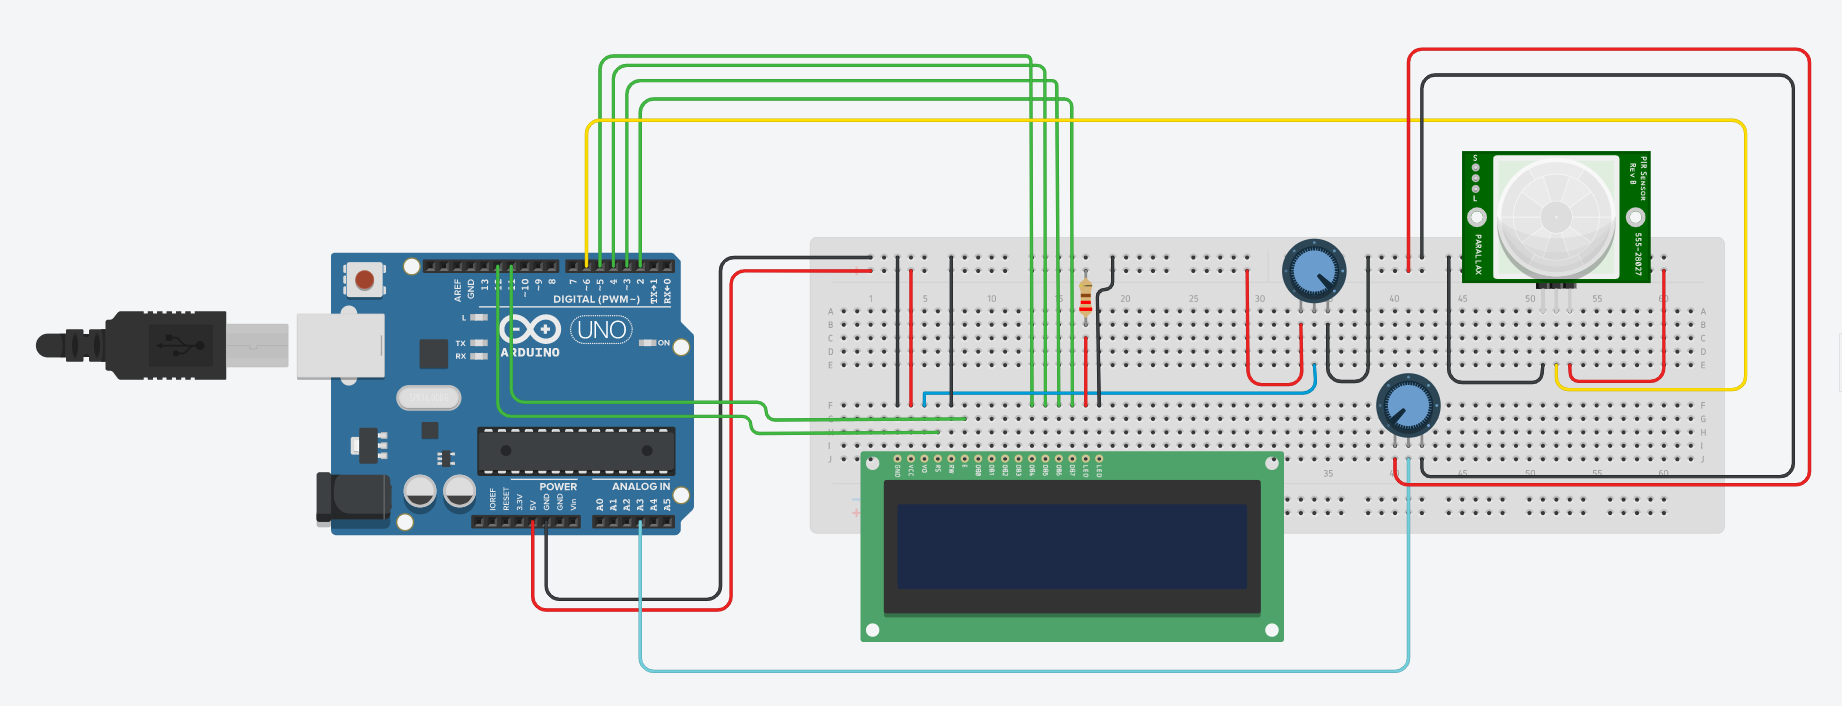
\includegraphics[width=\textwidth]{\LocPIRfig/propsys.png}
    \label{fig:propsys}
  \caption{Proposed system for motion detection for PIR Interfacing}
\end{figure} 

\section{PIR Sensor HC-SR501}
A passive infrared sensor is an electronic sensor that measures infrared light radiating from objects. PIR sensors mostly used in PIR-based motion detectors.
PIR sensor is specially designed to detect such levels of infrared radiation. It basically consists of two main parts: A Pyroelectric Sensor and A special lens called Fresnel lens which focuses the infrared signals onto the pyroelectric sensor.
A Pyroelectric Sensor actually has two rectangular slots in it made of a material that allows the infrared radiation to pass. Behind these, are two separate infrared sensor electrodes, one responsible for producing a positive output and the other a negative output. The reason for that is that we are looking for a change in IR levels and not ambient IR levels. The two electrodes are wired up so that they cancel each other out. If one half sees more or less IR radiation than the other, the output will swing high or low.


\begin{figure}[hpt]
  \centering
    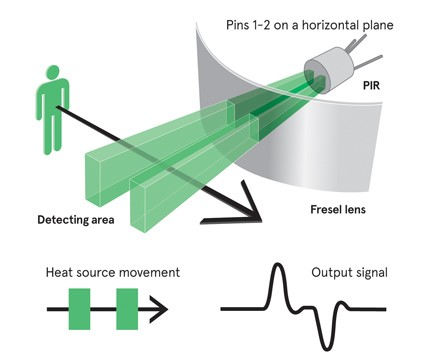
\includegraphics[width=\textwidth]{\LocPIRfig/pyrosensor.jpg}
    \label{fig:pyro} \hfill
  \caption{Pyroelectric Sensor}
\end{figure}


When the sensor is idle, i.e. there is no movement around the sensor; both slots detect the same amount of infrared radiation, resulting in a zero output signal.
But when a warm body like a human or animal passes by; it first intercepts one half of the PIR sensor, which causes a positive differential change between the two halves. When the warm body leaves the sensing area, the reverse happens, whereby the sensor generates a negative differential change. The corresponding pulse of signals results in the sensor setting its output pin high.

There are two potentiometers on the board to adjust a couple of parameters:
\begin{itemize}
  \item \textbf{Sensitivity}– This sets the maximum distance that motion can be detected. It ranges from 3 meters to approximately 7 meters. The topology of your room can affect the actual range you achieve.
  \item \textbf{Time}– This sets how long that the output will remain HIGH after detection. At minimum it is 3 seconds, at maximum it is 300 seconds or 5 minutes.
\end{itemize}
 
It has two settings:
\begin{itemize}
  \item 	H– This is the Hold/Repeat/Retriggering. In this position the HC-SR501 will continue to output a HIGH signal as long as it continues to detect   movement.
  \item  L– This is the Intermittent or No-Repeat/Non- Retriggering In this position the output will stay HIGH for the period set by the TIME potentiometer adjustment.
\begin{figure}[hpt]
  \centering
  \subfloat[No-Repeat/Non- Retriggering  charactiristics]{
    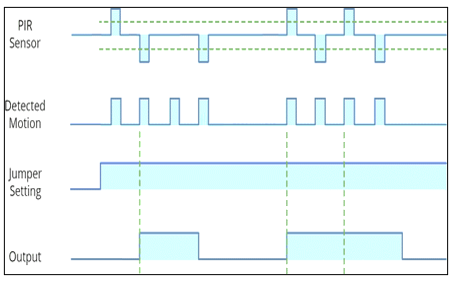
\includegraphics[width=\smfig]{\LocPIRfig/h.png}
    \label{fig:h}} \hfill
  \subfloat[Symbolic representation of an LDR]{
    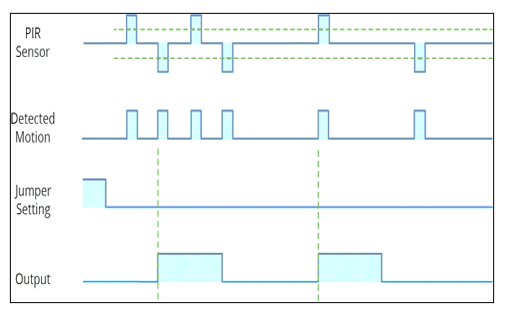
\includegraphics[width=\smfig]{\LocPIRfig/l.png}
    \label{fig:l}}
  \caption{Settings of PIR Sensor}
\end{figure}
\end{itemize}
\begin{figure}[hpt]
  \centering
    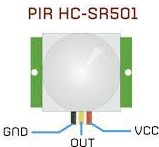
\includegraphics[width=\smfig]{\LocPIRfig/pirpinout.jpg}
    \label{fig:pinp} \hfill
  \caption{Pinout of PIR sensor}
\end{figure} 
\subsection{PIR sensor PINOUT}


\begin{itemize}
  \item \textbf{VCC} is the power supply for HC-SR501 PIR sensor which we connect the 5V pin on the Arduino.
  \item \textbf{Output} pin is a 3.3V TTL logic output. LOW indicates no motion is detected, HIGH means some motion has been detected.
  \item \textbf{GND} should be connected to the ground of Arduino.
\end{itemize}

\section{Interfacing the PIR through the Arduino IDE}
\label{sec:pir-arduino-code}
\label{sec:pir-arduino-code}
\subsection{Interfacing the PIR}
In this section, we shall describe how to read the voltage values from a HC-SR501 PIR Sensor connected to the digital pin 6 of the Arduino Uno board. The HC-SR501 PIR Sensor has to be connected to the Arduino Uno board before doing these experiments and the Arduino Uno needs to be connected to the computer with a USB cable, as shown in Fig 1.1.

\begin{enumerate}
  \item Read the digital value of PIR sensor as mentioned above using digitalRead function.
        \lstinputlisting[firstline=12,lastline=12]
        {\LocPIRardcode/pir/pir.ino}
\item The value received by digitalRead will be 0/1 (HIGH/LOW) depending upon whether motion is detected or not detected by PIR sensor. The received value is printed in serial monitor.
        \lstinputlisting[firstline=17,lastline=17]
        {\LocPIRardcode/pir/pir.ino}
\item Delay is added to slow down the rate of output being printed in serial monitor.
        \lstinputlisting[firstline=19,lastline=19]
        {\LocPIRardcode/pir/pir.ino}
The functions are written inside void loop and the operations will keep on working till the Arduino code executes.    

\end{enumerate}


\subsection{Arduino Code}
\label{sec:ldr-arduino-code}
\addtocontents{ard}{\protect\addvspace{\codclr}}

\begin{ardcode}
  \acaption{Read and display the PIR values}
  {Read and display the PIR values.  Available at
    \LocPIRardbrief{pir/pir.ino}.}
  \label{ard:ldr-read}
  \lstinputlisting{\LocPIRardcode/pir/pir.ino}
\end{ardcode}





\section{Interfacing the PIR through Python}
\subsection{Interfacing the PIR}
In this section, we discuss how to carry out the experiments of the section \secref{sec:pir-arduino-code} using Python. We will list the same experiment. The HC-SR501 should be attached to the Arduino Uno board before doing these experiments and the Arduino Uno needs to be connected to the computer with a USB cable, as shown in Fig 1.1 .The Firmware code given in appendix should be uploaded to the Arduino board. 

\begin{enumerate}
  \item Declare the pin used for the HC-SR501 using a variable and creating a counter variable. 
        \lstinputlisting[firstline=23,lastline=25]
        {\LocPIRpycode/PIR-FOSSEE.py} 
 \item The Python command used for digitalRead function is, 
        \lstinputlisting[firstline=27,lastline=27]
        {\LocPIRpycode/PIR-FOSSEE.py} 
 \item The output Motion detected, Motion ended and No Motion are printed based on the input received      from PIR sensor and the pirstate variable. Initially pirstate is 0, and until the input from the Sensor is 1(High), the output printed in python screen will be “No Motion”. Once the Sensor detects motion(give input 1), pirstate is changed to 1 and the output “Motion detected” is printed. Then once the input becomes 0(LOW), the output printed on python screen will be “Motion Ended”.
        \lstinputlisting[firstline=29,lastline=37]
        {\LocPIRpycode/PIR-FOSSEE.py} 

\end{enumerate}



\subsection{Python Code}
\label{sec:ldr-python-code}
\addtocontents{pyd}{\protect\addvspace{\codclr}}

\begin{pycode}
  \pcaption{Read and display the PIR values}
  {Read and display the LDR values.  Available at
    \LocPIRpybrief{PIR-FOSSEE.py}.}
  \label{py:ldr-read}
  \lstinputlisting{\LocPIRpycode/PIR-FOSSEE.py}
\end{pycode}



\section{16x2 LCD}
\begin{figure}[hpt]
  \centering
    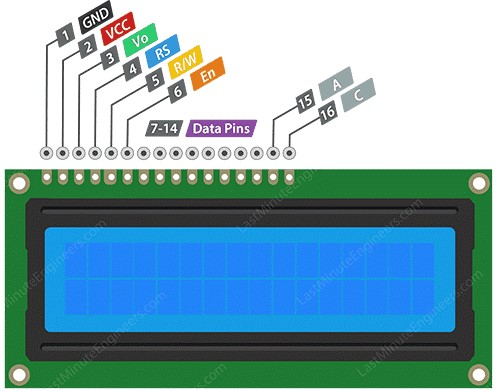
\includegraphics[width=\textwidth]{\LocPIRfig/lcdpinout.jpg}
    \label{fig:pinlcd} \hfill
  \caption{Pinout of 16x2 LCD}
\end{figure} 

\begin{itemize}
  \item \textbf{GND} should be connected to the ground of Arduino.
  \item \textbf{VCC} is the power supply for the LCD which we connect the 5 volts pin on the Arduino
  \item \textbf{Vo (LCD Contrast) } controls the contrast and brightness of the LCD. Using a simple voltage divider with a potentiometer, we can make fine adjustments to the contrast.
  \item \textbf{RS (Register Select) }  pin lets the Arduino tell the LCD whether it is sending commands or the data. Basically, this pin is used to differentiate commands from the data.
For example, when RS pin is set to LOW, then we are sending commands to the LCD (like set the cursor to a specific location, clear the display, scroll the display to the right and so on). And when RS pin is set on HIGH we are sending data/characters to the LCD.
  \item \textbf{R/W (Read/Write) } pin on the LCD is to control whether or not you’re reading data from the LCD or writing data to the LCD. Since we’re just using this LCD as an OUTPUT device, we’re going to tie this pin LOW. This forces it into the WRITE mode.
  \item \textbf{E (Enable) } pin is used to enable the display. Meaning, when this pin is set to LOW, the LCD does not care what is happening with R/W, RS, and the data bus lines; when this pin is set to HIGH, the LCD is processing the incoming data.
  \item \textbf{D0-D7 (Data bus) } are the pins that carries the 8 bit data we send to the display. For example, if we want to see the uppercase ‘A’ character on the display we will set these pins to 0100 0001(according to the ASCII table) to the LCD.
  \item \textbf{A-K (Anode \& Cathode) } pins are used to control the backlight of the LCD.
\end{itemize}


\section{Interfacing the PIR \& LCD through the Arduino IDE}
\label{sec:pir-lcd-arduino-code}
\subsection{Interfacing the PIR \& LCD}
Controlling LCD is a quite complicated task. Fortunately, thanks to the LiquidCrystal library, this library simplifies the process of controlling LCD for you so we don't need to know the low-level instructions. We just need to connect Arduino to LCD and use the functions of the library.

\begin{enumerate}
  \item Include the library: 
        \lstinputlisting[firstline=1,lastline=1]
        {\LocPIRardcode/pir-lcd/pir-lcd.ino}
\item Creates an LCD object with parameters: (rs, enable, d4, d5, d6, d7)
        \lstinputlisting[firstline=4,lastline=4]
        {\LocPIRardcode/pir-lcd/pir-lcd.ino}
\item Set up the LCD's number of columns and rows and clear the lcd screen.
        \lstinputlisting[firstline=12,lastline=15]
        {\LocPIRardcode/pir-lcd/pir-lcd.ino}
\item 4.	The cursor is moved to the desired position, and the output “No motion”, “Motion detected!” and “Motion ended” are displayed on the LCD.
        \lstinputlisting[firstline=20,lastline=39]
        {\LocPIRardcode/pir-lcd/pir-lcd.ino}
 

\end{enumerate}


\subsection{Arduino Code}
\label{sec:ldr-arduino-code}
\addtocontents{ard}{\protect\addvspace{\codclr}}

\begin{ardcode}
  \acaption{Read and display the PIR values in LCD}
  {Read and display the PIR values.  Available at
    \LocPIRardbrief{pir-lcd/pir-lcd.ino}.}
  \label{ard:ldr-read}
  \lstinputlisting{\LocPIRardcode/pir-lcd/pir-lcd.ino}
\end{ardcode}





\section{Interfacing the PIR \& LCD through Python}
\subsection{Interfacing the PIR \& LCD}
In this section, we discuss how to carry out the experiments of the \secref{sec:pir-lcd-arduino-code} from Python. We will list the same experiment. The LCD should be attached to the Arduino Uno board before doing these experiments and the Arduino Uno needs to be connected to the computer with a HC-SR501 PIR Sensor USB cable, as shown in Fig 1.1  The Firmware code given in appendix should be uploaded to the Arduino board.

\begin{enumerate}
  \item  Declare the pin used for the HC-SR501 using a variable and creating a counter variable pirstate and 3 variable nomot, motdet and motend for being used in the function from Step 2.
        \lstinputlisting[firstline=24,lastline=28]
        {\LocPIRpycode/pir-lcd.py} 
 \item The python-based command to print the “Motion detected!”, “Motion ended!” and “No Motion!” are given below respectively.
        \lstinputlisting[firstline=4,lastline=4]
	{\LocPIRpycode/pir-lcd.py} 
 \item Set up the LCD's number of columns and rows and clear the lcd screen.
        \lstinputlisting[firstline=33,lastline=33]
	{\LocPIRpycode/pir-lcd.py}
	\lstinputlisting[firstline=37,lastline=37]
	{\LocPIRpycode/pir-lcd.py}
	\lstinputlisting[firstline=41,lastline=41]
        {\LocPIRpycode/pir-lcd.py} 

\end{enumerate}



\subsection{Python Code}
\label{sec:ldr-python-code}
\addtocontents{pyd}{\protect\addvspace{\codclr}}

\begin{pycode}
  \pcaption{Read and display the PIR values in LCD}
  {Read and display the LDR values.  Available at
    \LocPIRpybrief{pir-lcd.py}.}
  \label{py:ldr-read}
  \lstinputlisting{\LocPIRpycode/pir-lcd.py}
\end{pycode}

\section{Setup \& Output}
\begin{figure}[hpt]
  \centering
    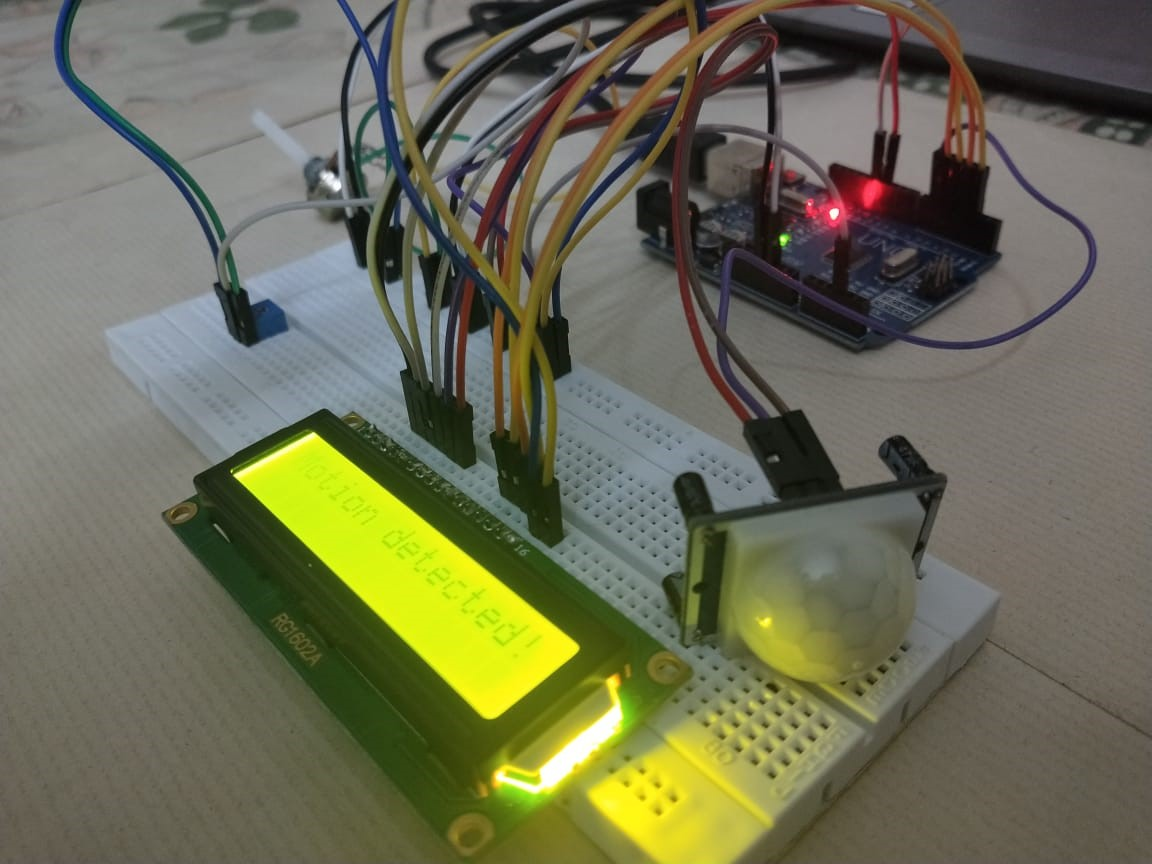
\includegraphics[width=\textwidth]{\LocPIRfig/setup1.jpg}
    \label{fig:set1} \hfill
  \caption{Setup 1}
\end{figure}
\begin{figure}[hpt]
  \centering
    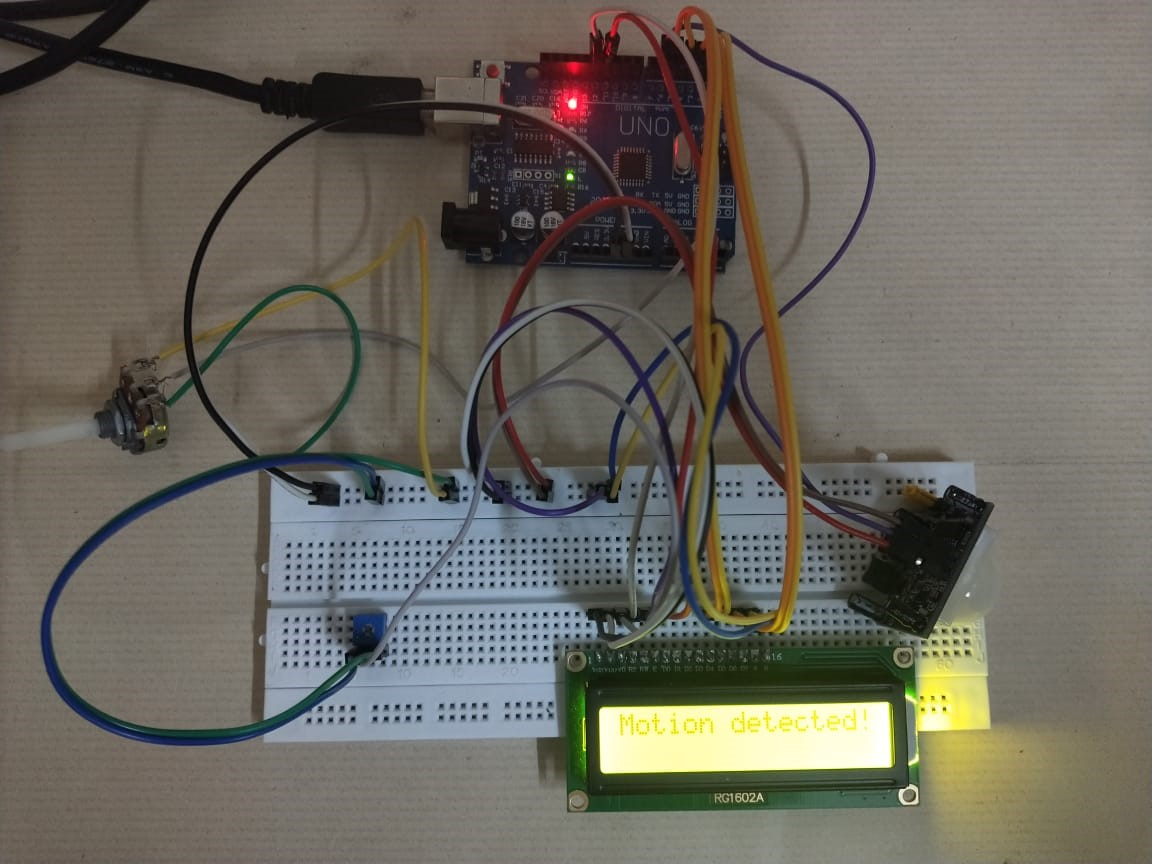
\includegraphics[width=\textwidth]{\LocPIRfig/setup2.jpg}
    \label{fig:set2} \hfill
  \caption{Setup 2}
\end{figure}
\begin{figure}[hpt]
  \centering
    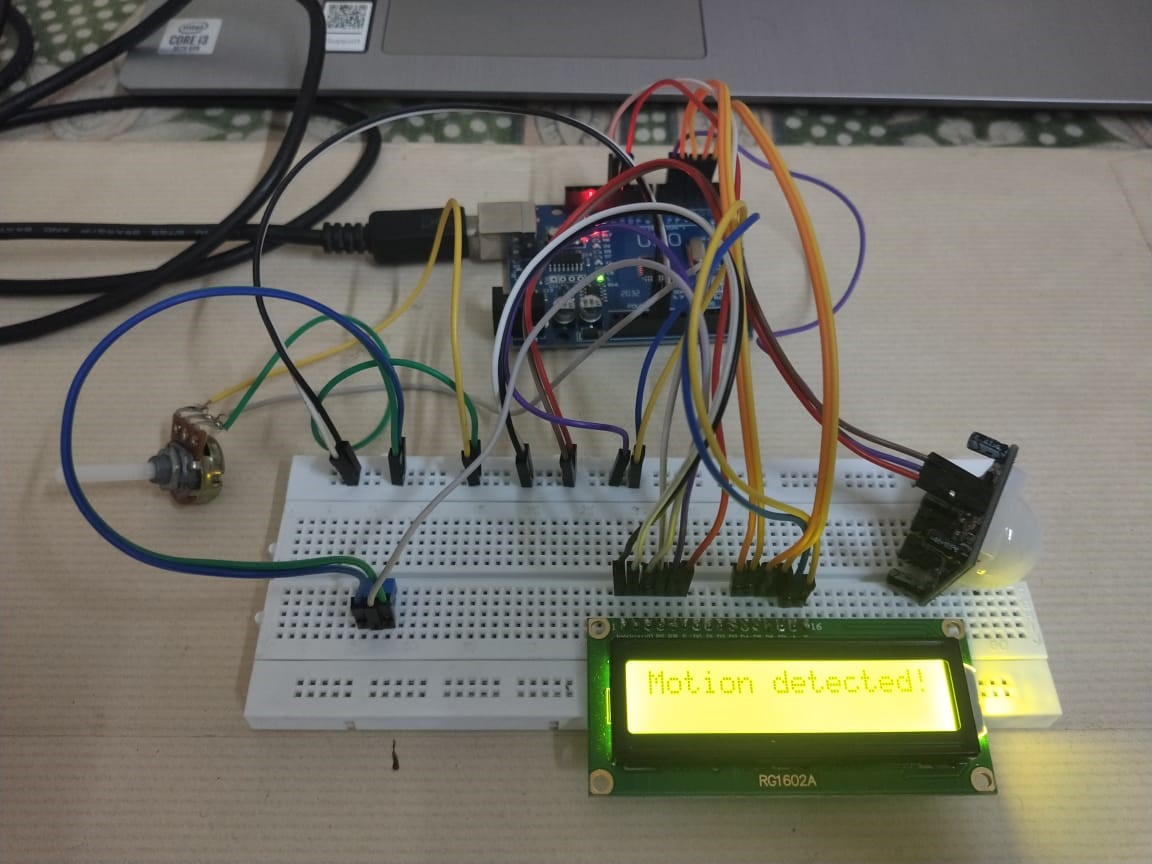
\includegraphics[width=\textwidth]{\LocPIRfig/setup3.jpg}
    \label{fig:set3} \hfill
  \caption{Setup 3}
\end{figure}
\begin{figure}[hpt]
  \centering
    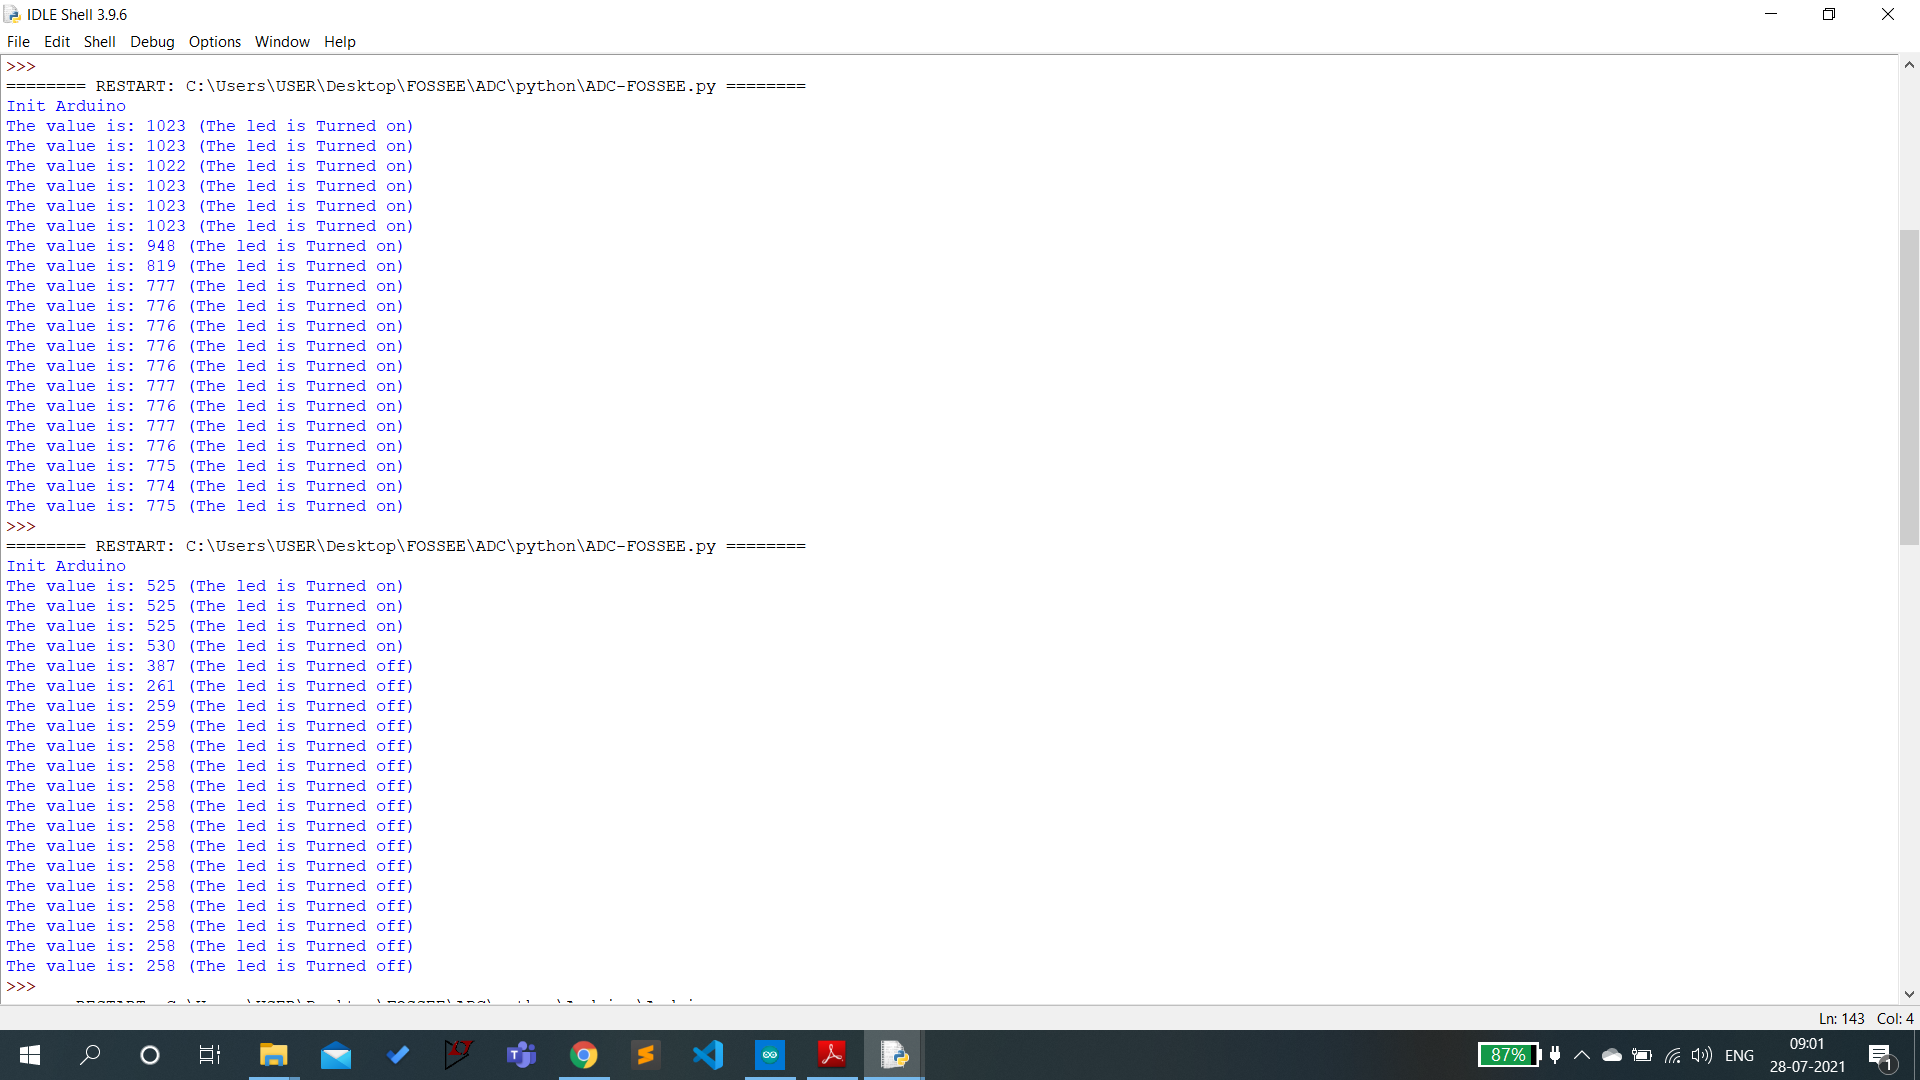
\includegraphics[width=\textwidth]{\LocPIRfig/output1.png}
    \label{fig:out1} \hfill
  \caption{Output 1}
\end{figure}
\begin{figure}[hpt]
  \centering
    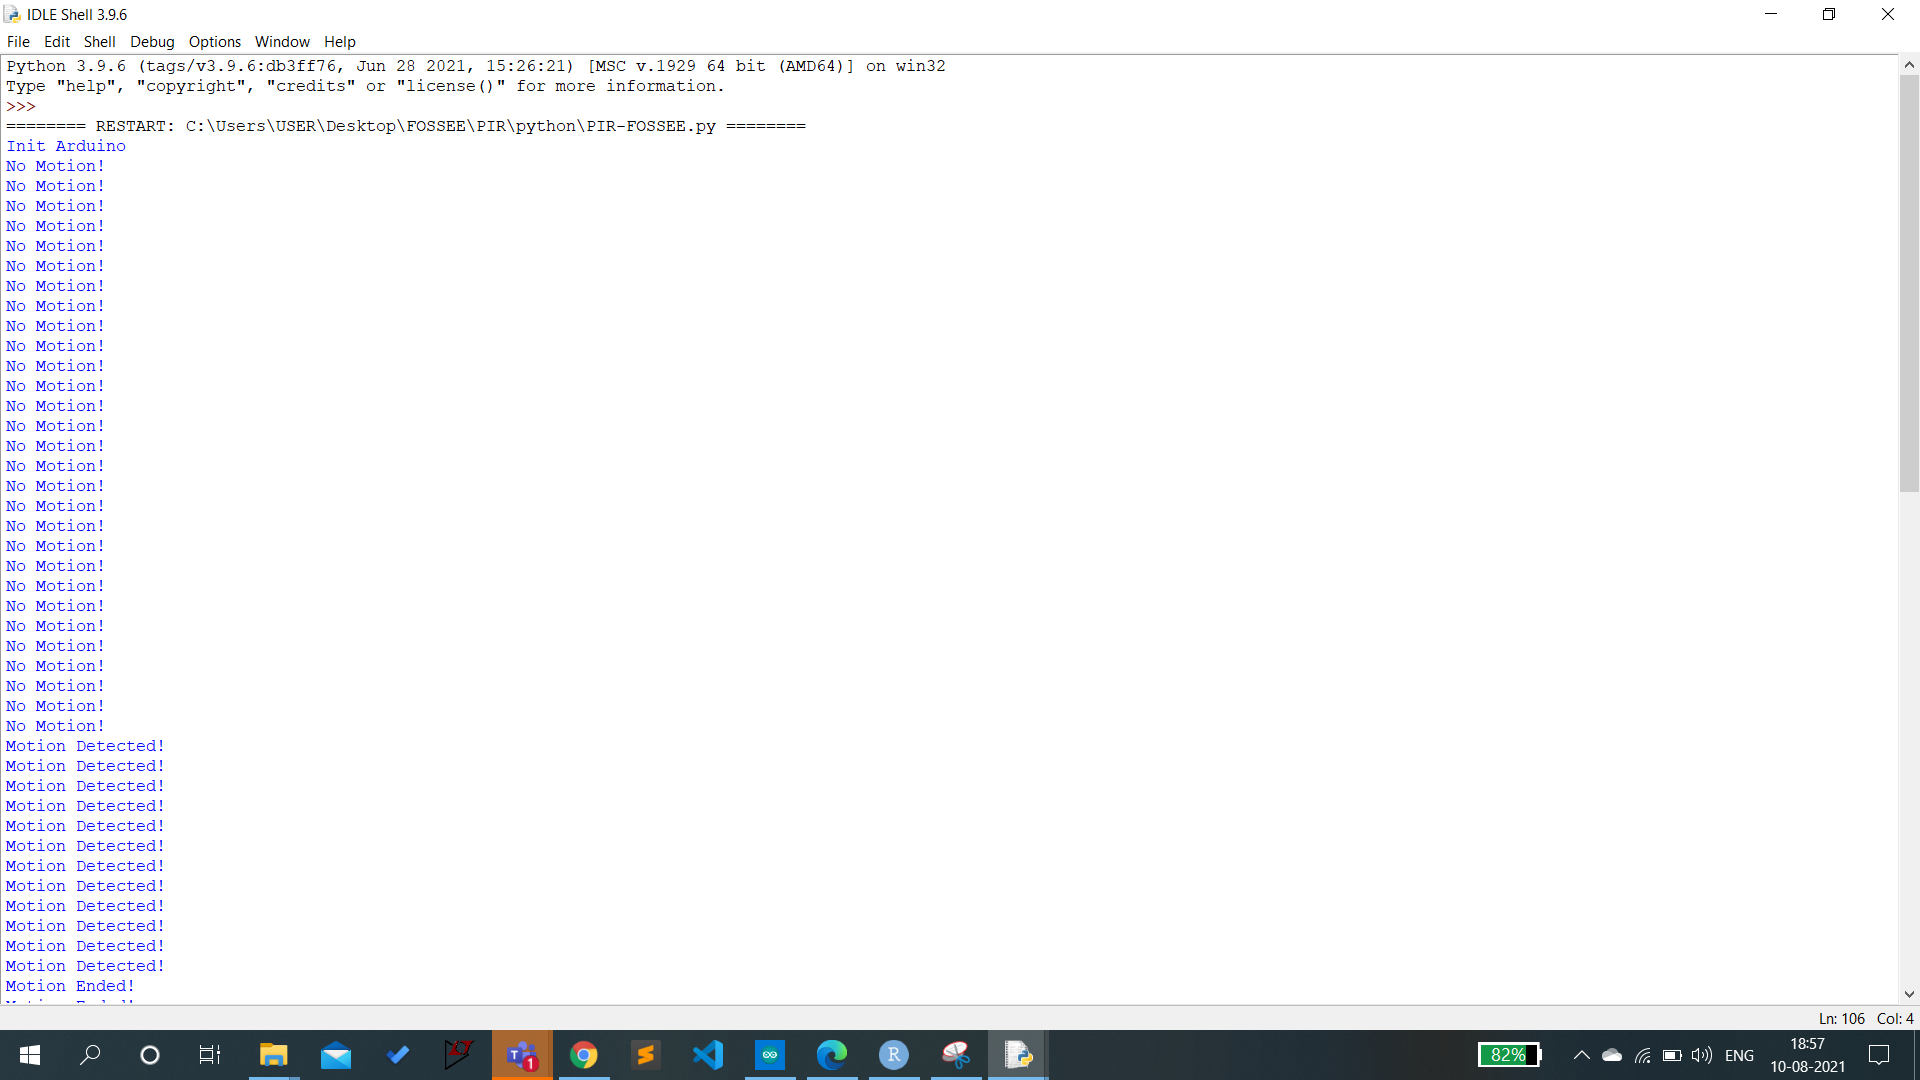
\includegraphics[width=\textwidth]{\LocPIRfig/output2.png}
    \label{fig:out2} \hfill
  \caption{Output 2}
\end{figure}















%\input{texfiles/microcontintro.tex}
%\input{texfiles/sciaurint.tex}
% \input{user-code/sw-env/sw-env.tex}





%\input{texfiles/servo.tex}
%\input{texfiles/Appendix.tex}
%\appendix
%\input{texfiles/sp-appendix.tex}
%\input{windows/windows}

\bibliography{bibliography.bib}
%\printindex
%\input{texfiles/AuthorInfo.tex}
\end{document}
